\chapter{Formal Analysis using Alloy}
This section provides a formal specification of the entire model using the Alloy language. We will use Alloy 6 to describe entities and relationships in systems. We choose Alloy 6 because is suited for modeling and analyzing the properties of software systems to ensure correctness and consistency.

\section{ Code}
\begin{lstlisting}
open util/relation
open util/boolean

//----SIGNATURES----
// User's role: it can be a student or a company
abstract sig Role {}
sig Student extends Role {
	applications: some Application,
	cv: one CV
}
sig CV{}
sig Company extends Role {
	postings: some Internship
}

// Users' personal information
sig User {
	email: one Email,
    	otherInformation: one PersonalData,
    	role: one Role
}
sig Email{}
sig PersonalData{}

// Internship
sig Internship {
	postedBy: one Company,
    	applicants: some Application,
    	description: one Description,
}
sig Description{}

// Application for an internship
sig Application {
	submittedBy: one Student,
    	relatedTo: one Internship,
    	interviews: one Interview,
   	var status:  Status
}
enum Status {Pending, Accepted, Rejected}

// Interview
sig Interview {
	schedule: one DateTime,
    	var outcome:  Outcome
}
enum Outcome {Passed, Failed, InProgress}
sig DateTime{}

//----FACTS----
// No two Users can have the same email or personal info
fact UniqueUsersEmailsAndPersonalInfo {
	all u1, u2: User | u1 != u2 implies
    		u1.email != u2.email and
    		u1.otherInformation != u2.otherInformation
}

// A role can only be associated with one User
fact OneUserPerStudentAndCompany{
	all s: Student | one u: User | 
		s in u.role 
	and
    	all c: Company |  one u: User | 
		c in u.role 
}

//DoubleArrowConstraint
fact DoubleAssociation {
	//An application can only be associated with a student
    	all a: Application | one s: Student | 
    		s in a.submittedBy and 
		a in s.applications and
    		s.applications.submittedBy=s 
    	//An application can only be associated with a Intenship
    	all a: Application | one i: Internship | 
    		a in i.applicants and  
		i in a.relatedTo and
    		i.applicants.relatedTo = i
    	//An internship can only be associated with a Company
    	all  i:Internship | one c: Company | 
    		c in i.postedBy and 
		i in c.postings and 
    		c.postings.postedBy = c  
}

//Unique Description, CV, and Interview 
fact UniqueItems {
	//description
    	all i1, i2: Internship | i1 != i2 implies
   		i1.description != i2.description
    	all dd: Description | one ii:Internship | 
		dd in ii.description
	//CV
    	all s1,s2: Student| s1 != s2 implies
		s1.cv != s2.cv
    	all ccvv:CV | one ss: Student |  
		ccvv in ss.cv
    	//interview
   	 all a1,a2: Application | a1!=a2 implies 
   		a1.interviews != a2.interviews
    	all i: Interview | one a: Application |
		 i in a.interviews
}

//Unique Application
fact UniqueApplications{
	all i1, i2: Internship | i1 != i2 implies 
    		#(i1.applicants & i2.applicants) <= 0
    	all c1, c2: Company | c1 != c2 implies 
    		#(c1.postings & c2.postings) <= 0
    	all s1,s2: Student | s1 !=s2 implies 
    		#(s1.applications & s2.applications) <=0
}

// A student can make only an application for one internship
fact UniqueApplicationsPerStudent {
	all s: Student | all i: Internship | 
    		#(s.applications & i.applicants) <= 1
}

//A role cannot have a mettengs the same day
fact SameDayMeetings {
	all ss1,ss2: Student | all cc1,cc2: Company |
   	all a1,a2: Application | a1!=a2 and
   		((ss1 in a1.submittedBy and 
		   ss2 in a2.submittedBy and
   		   cc1 in a1.relatedTo.postedBy and
		   cc1 in a1.relatedTo.postedBy)
   	or
   		 (ss1 in a1.submittedBy and 
		  ss1 in a2.submittedBy and
   		  cc1 in a1.relatedTo.postedBy and 
		  cc2 in a1.relatedTo.postedBy))
   	implies a1.interviews.schedule != a2.interviews.schedule
}

// Interview process
fact InterviewProess{ 
	all a: Application | 
        	always( a.interviews.outcome = InProgress 
			implies a.status = Pending)
	 	and always(a.interviews.outcome = Passed 
			implies a.status = Accepted)
		and always(a.interviews.outcome = Failed 
			implies a.status = Rejected)
}

\end{lstlisting}



\section{ Models}
\subsection{Static Analysis}
\textbf{[MS1]} The model shows the basic scenario where one student is applying for an internship at a company with pending status and an in-progress interview.
\begin{lstlisting}
//one student and one company
pred oneStudentOneCompanyOneInternship {
    #Student = 1
    #Company = 1
    #Internship = 1
}
run oneStudentOneCompanyOneInternship for 2
\end{lstlisting}
\textit{ \#6:Instance found oneStudentOneCompanyOneInternship is consistent.}
\begin{figure}[H]
    \centering
    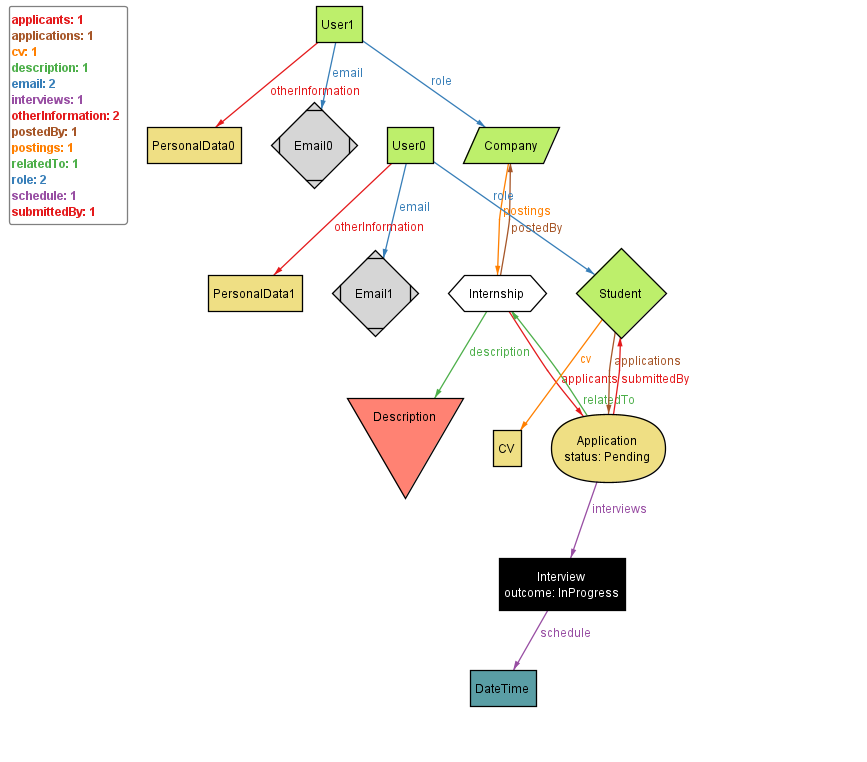
\includegraphics[width=0.75\linewidth]{RASD//Images/1st1com.png}
    \caption{1 Student, 1 Company, 1 Internship}
    \label{fig:enter-label}
\end{figure}

\textbf{[MS2]} The model shows a scenario where two students are applying for an internship at a company with pending status and an in-progress interview.
\begin{lstlisting}
//two students and one company
pred twoStudentOneCompanyOneInternship {
    #Student = 2
    #Company = 1
    #Internship = 1
}
run twoStudentOneCompanyOneInternship for 3
\end{lstlisting}
\textit{ \#7:Instance found twoStudentOneCompanyOneInternship is consistent.}
\begin{figure}[H]
    \centering
    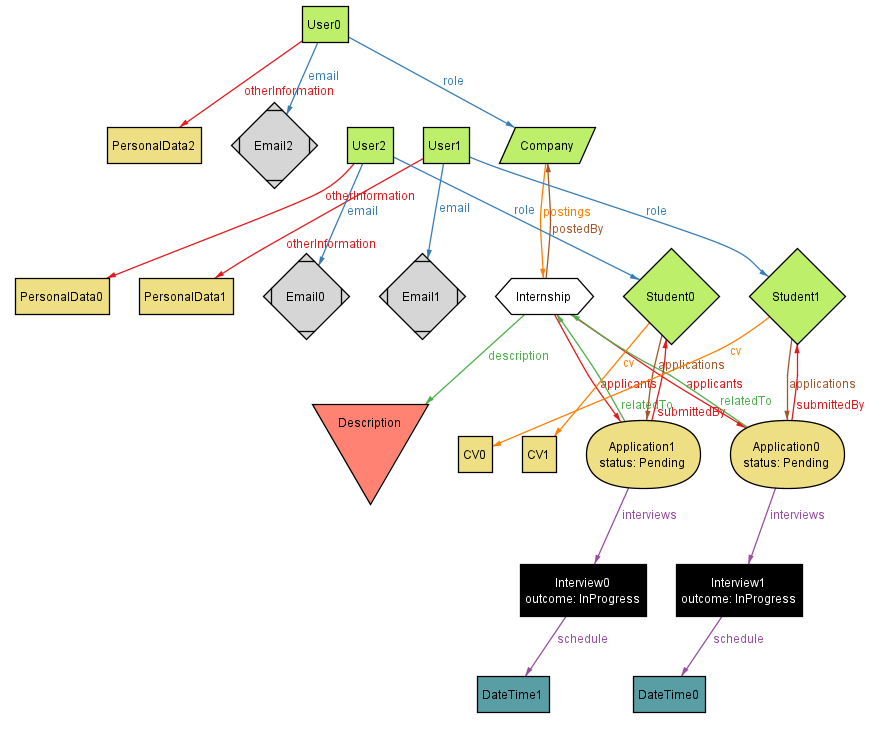
\includegraphics[width=1\linewidth]{RASD//Images/2st1com.png}
    \caption{2 Student, 1 Company, 1 Internship}
    \label{fig:enter-label}
\end{figure}

\textbf{[MS3]} The model shows a scenario where one student is applying for three internships 2 at company A and one at company B with pending status and an in-progress interview.
\begin{lstlisting}
//one student and one two companies
pred oneStudentTwoCompanyThreeInternship {
    #Student = 1
    #Company = 2
    #Internship = 3
}
run oneStudentTwoCompanyThreeInternship for 3 
\end{lstlisting}
{ \#8:Instance found oneStudentTwoCompanyThreeInternship is consistent.}
\begin{figure}[H]
    \centering
    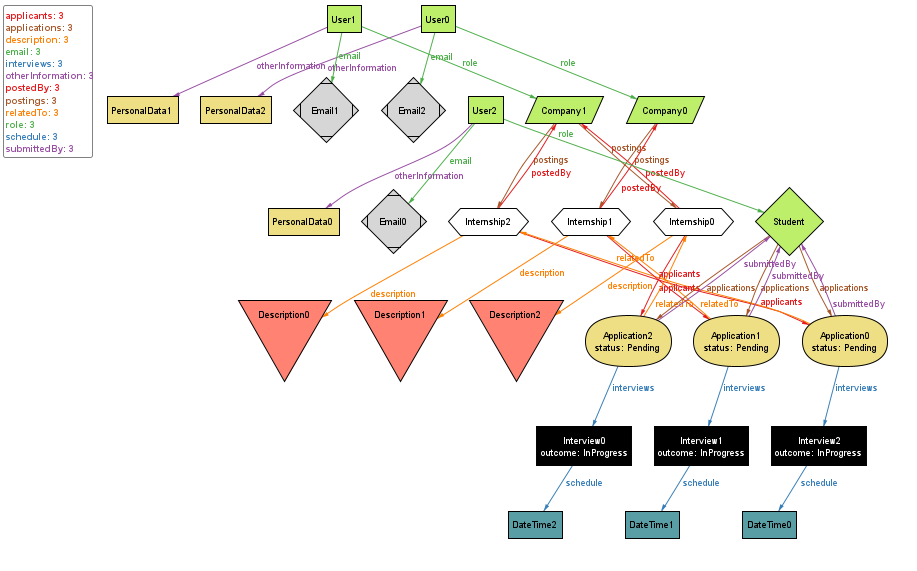
\includegraphics[width=1\linewidth]{RASD//Images/1st2com.png}
    \caption{1 Student, 1 Company, 3 Application}
    \label{fig:enter-label}
\end{figure}
\begin{figure}[H]
    \centering
    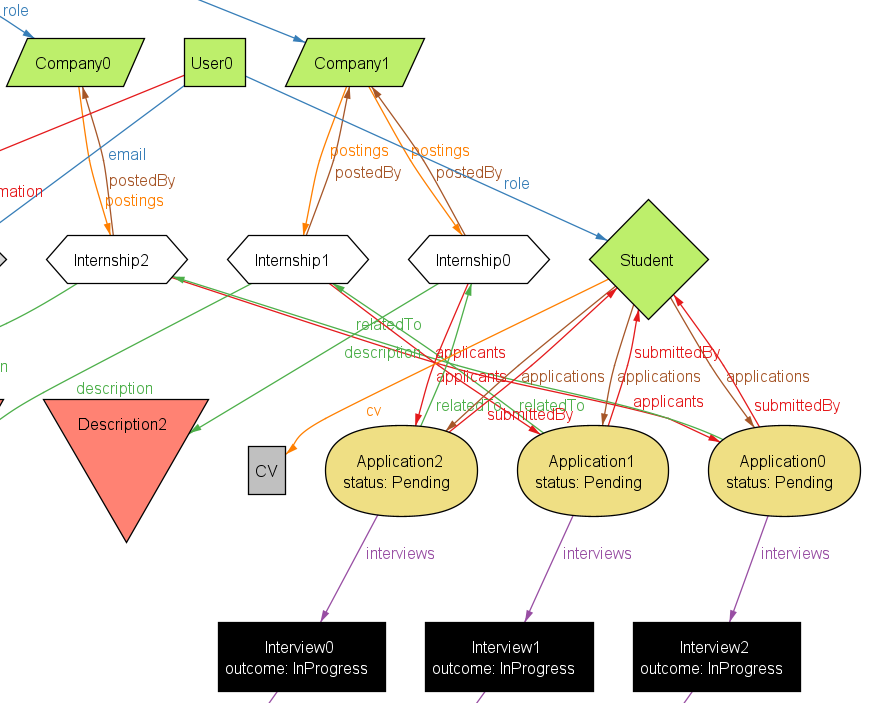
\includegraphics[width=0.75\linewidth]{RASD//Images/1st2comzoom.png}
    \caption{1 Student, 1 Company, 3 Application - zoom on the relations}
    \label{fig:enter-label}
\end{figure}

\subsection{Dynamic Analysis}
\textbf{[MD1]}The model shows the basic scenario where one student applies for an internship
at a company. The dynamic analysis shows how the positive interview status influences the application outcome.

If InProgress $=>$ Passed then Pending $=>$ Accepted
\begin{lstlisting}
//passed interview
pred interviewPassed[ap:Application, s:Student, c:Company]{
	ap.interviews.outcome = InProgress ; 
	ap.interviews.outcome = Passed
	#Student = 1
    	#Company = 1
    	#Internship = 1
}
run interviewPassed for 2  
\end{lstlisting}
{ \#9:Instance found interviewPassed is consistent.}
\begin{figure}[H]
    \centering
    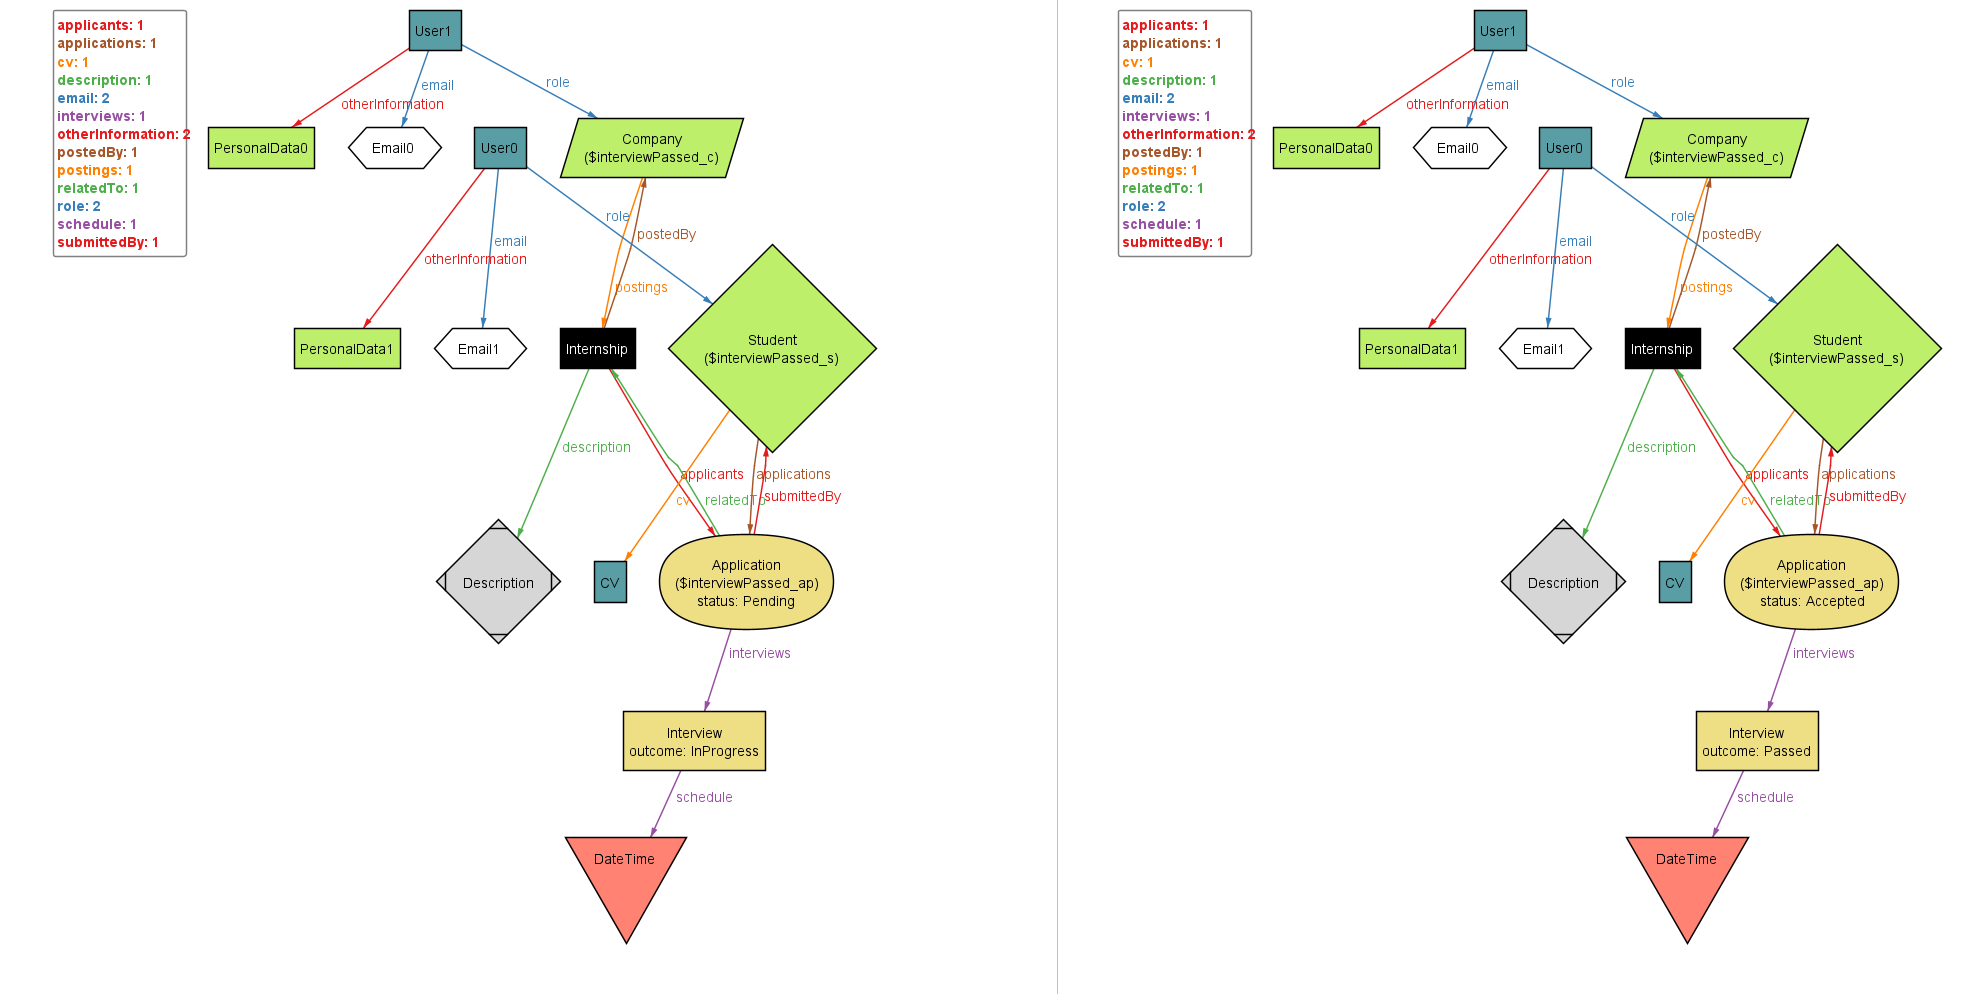
\includegraphics[width=1\linewidth]{RASD//Images/passed.png}
    \caption{Passed inteview}
    \label{fig:enter-label}
\end{figure}

\textbf{[MD2]}The model shows the basic scenario where one student applies for an internship
at a company. The dynamic analysis shows how the negative interview status influences the application outcome.

If InProgress $=>$ Failed then Pending $=>$ Rejected
\begin{lstlisting}

//failed interview
pred interviewRejected[ar:Application, s:Student, c:Company]{
	ar.interviews.outcome = InProgress ; 
	ar.interviews.outcome = Failed
	#Student = 1
    	#Company = 1
    	#Internship = 1
}
run interviewRejected for 2 
\end{lstlisting}
{ \#10:Instance found interviewRejected is consistent.}
\begin{figure}[H]
    \centering
    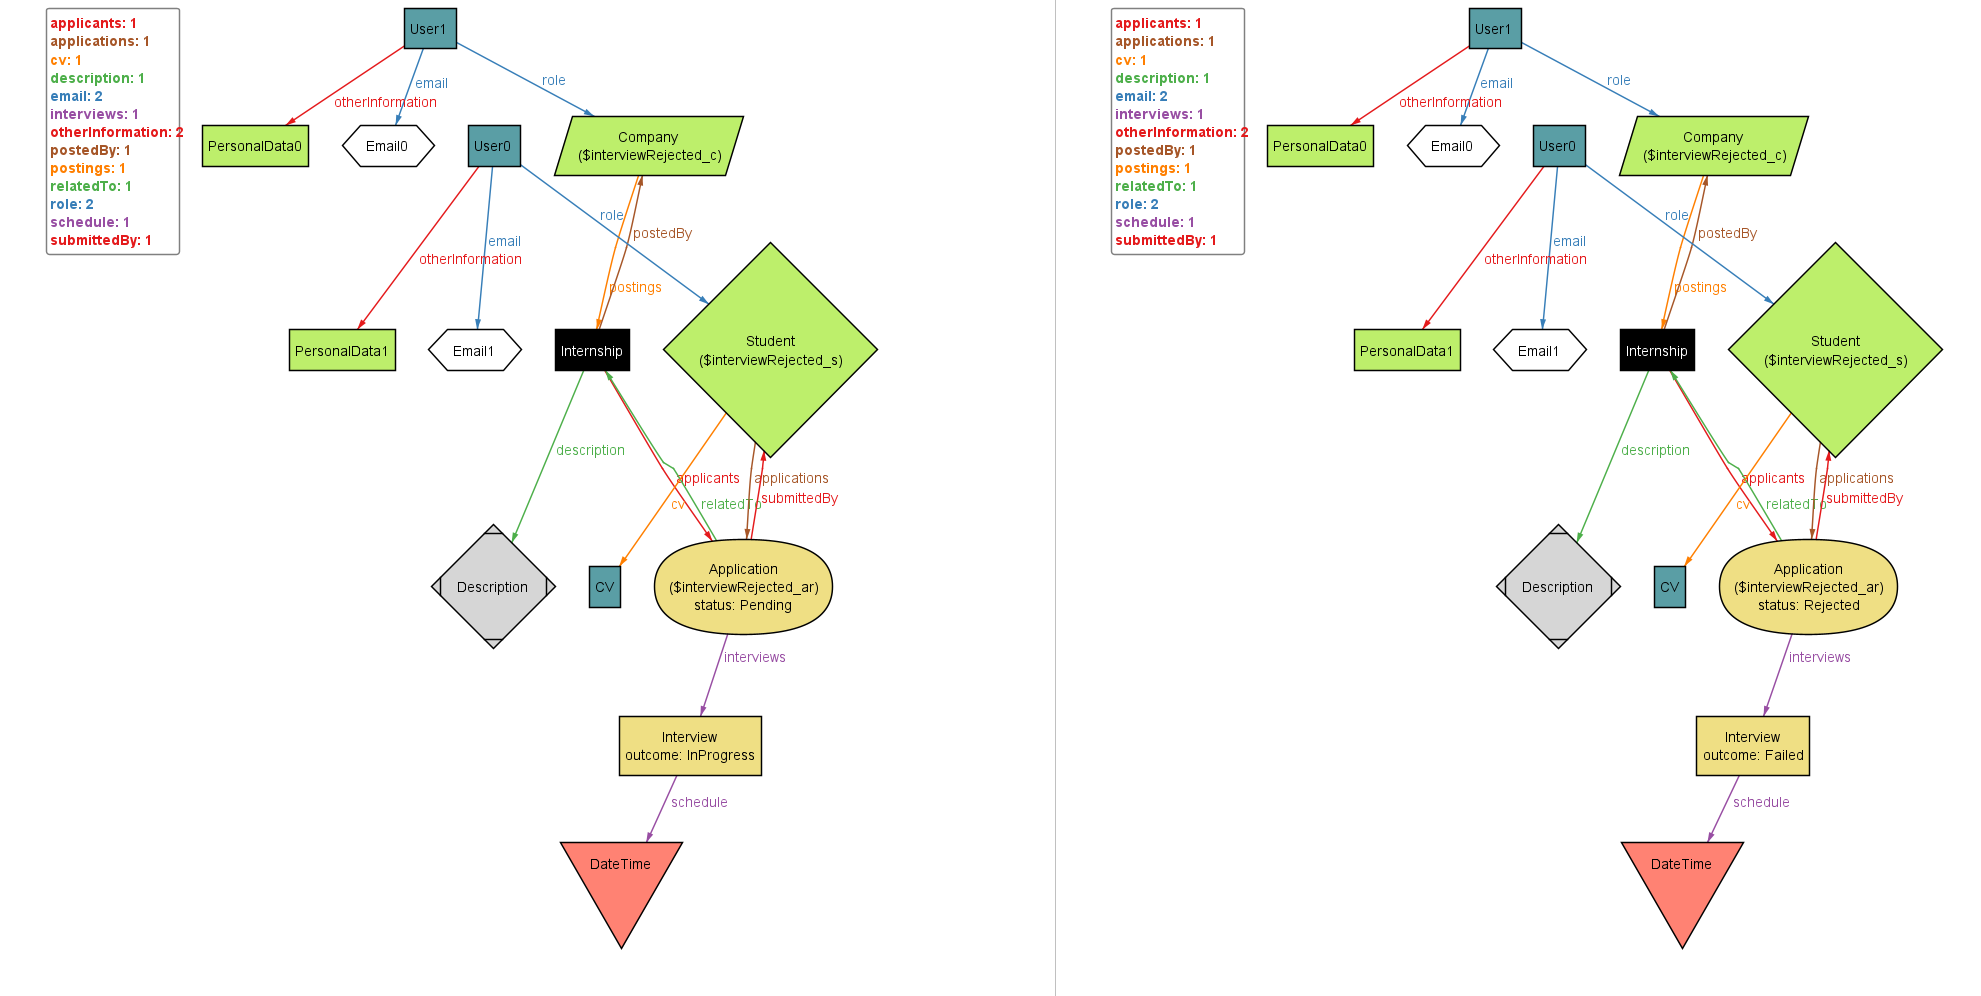
\includegraphics[width=1\linewidth]{RASD//Images/failed.png}
    \caption{Failed interview}
    \label{fig:enter-label}
\end{figure}

\section{ Assertions}
\textbf{[A1]} Assertion to verify the correctness of the user structure as:
\begin{itemize}
    \item No Users will have the same email or the Personal info
    \item Each role can only be associated with one User
\end{itemize}
\begin{lstlisting}
// Assertion to verify the correctness of the user structure as:
assert VerifyUserStructure{
	//mail and personal info
    	all u1, u2: User | u1 != u2 implies 
    		u1.email != u2.email and  
		u1.otherInformation != u2.otherInformation
	//role
    	all s: Student | one u: User | u.role = s
    	all c: Company | one u: User | u.role = c
}
check VerifyUserStructure
\end{lstlisting}
\textit{\#1: VerifyUserStructure may be valid.}


\textbf{[A2]} Assertion to verify DoubleArrowConstraint:
\begin{itemize}
    \item An application can only be associated with a student
    \item An application can only be associated with a Intenship
    \item An internship can only be associated with a Company
\end{itemize}
\begin{lstlisting}
//Assertion to verify DoubleArrowConstraint
assert VerifyDoubleAssociation {
	//An application can only be associated with a student
    	all a: Application | one s: Student | 
    	s in a.submittedBy and a in s.applications and
    	s.applications.submittedBy=s
    	//An application can only be associated with a Intenship
    	all a: Application | one i: Internship | 
    	a in i.applicants and  i in a.relatedTo and
    	i.applicants.relatedTo = i
    	//An internship can only be associated with a Company
    	all  i:Internship | one c: Company | 
    	c in i.postedBy and i in c.postings and 
    	c.postings.postedBy = c  
}
check VerifyDoubleAssociation
\end{lstlisting}
\textit{\#2: VerifyDoubleAssociation may be valid.}


\textbf{[A3]} Assertion to verify all Internship application structure
\begin{itemize}
    \item Unique Description, CV, and Interview 
    \item Unique Application
    \item A student can make only an application for one internship
\end{itemize}
\begin{lstlisting}
// Assertion to verify all Internship application structure
assert VerifyInternshipStructures {
	//Unique Description, CV, and Interview 
    	all i1, i2: Internship | i1 != i2 implies 
		i1.description != i2.description
    	all dd: Description | one ii:Internship | 
		dd in ii.description
    	all s1,s2: Student| s1 != s2 implies s1.cv != s2.cv
    	all ccvv:CV | one ss: Student |  ccvv in ss.cv
    	all a1,a2: Application | a1!=a2 implies 
		a1.interviews != a2.interviews
    	all i: Interview | one a: Application |
		i in a.interviews
    	//Unique Application
   	 all i1, i2: Internship | i1 != i2 implies 
   	#(i1.applicants & i2.applicants) <= 0
   	all c1, c2: Company | c1 != c2 implies 
   	#(c1.postings & c2.postings) <= 0
   	all s1,s2: Student | s1 !=s2 implies 
    	#(s1.applications & s2.applications) <=0
   	////Student can make only 1 application for 1 internship
    	all s: Student | all i: Internship | 
    	#(s.applications & i.applicants) <= 1
}
check VerifyInternshipStructures
\end{lstlisting}
\textit{\#3: VerifyInternshipStructures may be valid}


\textbf{[A4]} Assertion to verify all Internship meeting schedules. Two meetings cannot be on the same day if:
\begin{itemize}
    \item are carried by the same company
    \item are carried by the same student
\end{itemize}
Therefore meetings have a schedule if they are submitted by a student
\begin{lstlisting}
//Two meetings cannot be in the same day if:
assert VerifyInterviewStructures {
	all ss1,ss2: Student | all cc1,cc2: Company |
   	all a1,a2: Application | a1!=a2 and
		//are carried by the same company
   		((ss1 in a1.submittedBy and 
		   ss2 in a2.submittedBy and
   		   cc1 in a1.relatedTo.postedBy and
		   cc1 in a1.relatedTo.postedBy)
   	or
		//are carried by the same student
   		 (ss1 in a1.submittedBy and 
		  ss1 in a2.submittedBy and
   		  cc1 in a1.relatedTo.postedBy and 
		  cc2 in a1.relatedTo.postedBy))
   	implies a1.interviews.schedule != a2.interviews.schedule
  	//meetings have a schedule if a student submits them
   	all a: Application | a.interviews.schedule != none 
   		 implies a.submittedBy in Student
}
check VerifyInternshipStructures
\end{lstlisting}
\textit{\#4: VerifyInterviewStructures may be valid}

\textbf{[A5]} Assertion to verify if the interview process is correctly related to the application process. Three cases are considered:
\begin{itemize}
    \item Failed $=>$ Rejected
    \item Passed $=>$ Accepted
    \item InProgress $=>$ Pending
\end{itemize}
\begin{lstlisting}
//Check interview process
assert InterviewProcess{
    all a: Application | 
	//Failed => Rejected
        some i: a.interviews | i.outcome = Failed 
		implies a.status = Rejected
	and 
	//Passed => Accepted
        some i: a.interviews | i.outcome = Passed 
		implies a.status = Accepted
	and
	//InProgress => Pending
        some i: a.interviews | i.outcome = InProgress 
		implies a.status = Pending
}
check InterviewProcess
\end{lstlisting}
\textit{\#5: InterviewProcess may be valid}